\section{Vorwort}

\subsection{Projektübersicht}
Im Projekt Oszi wird ein Oszilloskop mittels eines FPGAs zu realisieren. Das Oszilloskop soll ein Frequenzband von 0Hz bis 500kHz einlesen und einen Spannungsbereich von -20V bis +20V abdecken. Die Spannungskurfe soll über ein Computerprogramm graphisch ausgegeben werden. Über das Programm soll ebenfalls der Spannungs- und Zeitbereich der Ausgabe einzustellen sein. Das Oszilloskop solle triggerbar sein und Tastköpfe kalibrieren können. Das Projekt besteht aus drei Aufgabenbereichen, dem Analog-Front-End, der Datenverarbeitung mit dem FPGA und der Ausgabe am PC.
\subsection{Projektgruppe}
Das Team entstand im Zuge des Sommersemster-Projekts in der 4. Schulstufe am TGM. Gleiche Intressen, gutes technisches Wissen und Verständnis, sowie eine gute Harmonie unter den Fruppenmitgliedern führte zum Zusammenschluss. Die Projektgruppe ist geschlossen aus einer Klasse, der 4AHEL 2021 am TGM.
\begin{center}
\begin{tabular}[h]{c|c|c}
\multicolumn{3}{ c }{Projektteilnehmer}\\
\hline
\textbf{Radike} & \textbf{Sauer} & \textbf{Wolf}\\
Markus & Sauer & Benedict\\
\hline
Bild 1 &  \raisebox{-\height}{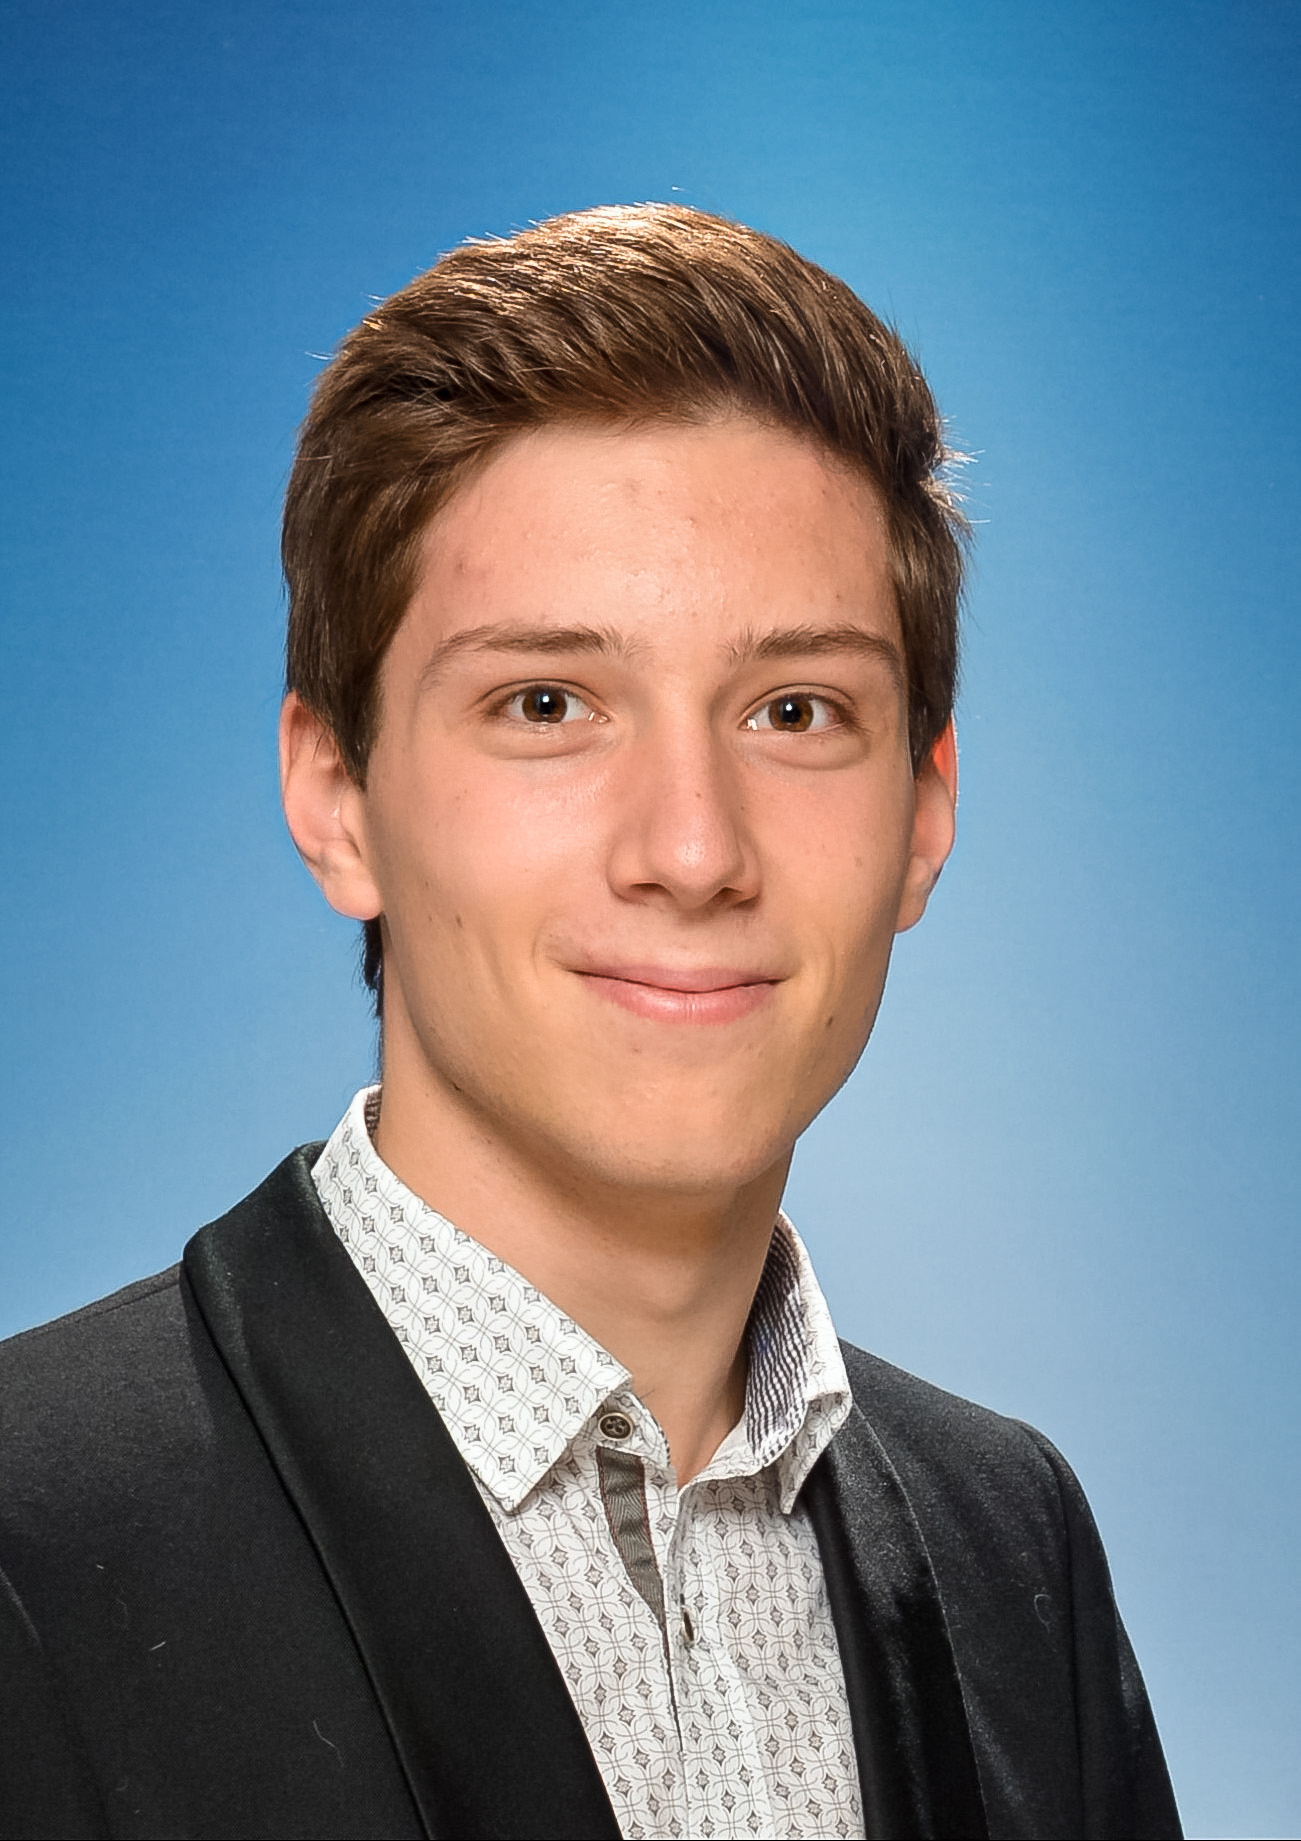
\includegraphics[width=4cm]{SAUER/Grafiken/FotoSauer.jpg}} & bild 3\\
\! & \! & \!\\
\hline
user interface & digital data processing & analog front end\\
\end{tabular}
\end{center}

\subsection{Projektbetreuer}
\begin{tabular}[h]{l|l}
		Fachbereich & Lehrperson\\
		\hline\hline
		Labor & GRÄBNER Kar-Heinz\\
		\hline
		Werkstatt & GRAUPE Andreas\\
	\end{tabular}
